\documentclass[../dissertation.tex]{subfiles}
\begin{document}
Instead of solving a discretised gradient flow equation (\ref{equ: Finite Difference Scheme for Curve Untangling Process}) directly,
a possible approach is to use approximation theory for a simple class of tangled curves;
if one knows beforehand that the initial curve is homeomorphic to a circle or a line segment,
it is possible to interpret and approximate the curve as comprised of simple functions,
and significantly optimise the untangling process by casting the functional reduction problem to
a traditional function reduction problem.
This also results in a simpler implementation for low-stake applications,
such as rope physics for video games.
Denote by $\mathbb{S}$ and $\mathbb{L}$ for bounded curves that are homeomorphic to a circle and a line segment, respectively, as in Appendix \ref{sct: Other Homeomorphism Classes}.

\subsubsection{Curves in $\mathbb{S}$}
For a continuous $2\pi$-periodic 1D function $f:\mathbb{R} \rightarrow \mathbb{R}$
(where one only needs to define $f$ on $\left[ 0,2\pi \right)$),
there exists a Fourier series representation:
\begin{align}
    f(x) &= \frac{a_0}{2} + \sum_{n=1}^{\infty} \left( a_n \cos {(nx)} + b_n \sin {(nx)} \right) \\
    &= \sum_{n=-\infty}^{\infty} c_n e^{inx}
\end{align}
where the two representations are equivalent.
The coefficients are given by
\begin{align}
    a_n &= \frac{1}{\pi} \int_{0}^{2\pi} f(x) \cos {\left( nx \right)} \intd x &\in \mathbb{R}\\
    b_n &= \frac{1}{\pi} \int_{0}^{2\pi} f(x) \sin {\left( nx \right)} \intd x &\in \mathbb{R} \\
    c_n &= \frac{1}{2 \pi} \int_{0}^{2\pi} f(x) e^{-inx} \intd x &\in \mathbb{C}
\end{align}

Now, for a vector-valued function such as a parameterised curve $\gammabf:\mathbb{R} \rightarrow \mathbb{R}^3$, one could write 3D Fourier series,
one for each coordinate (Figure \ref{fig: Fourier series decomposition into 1D}):
\begin{align}
    \mathbf{\gammabf} (t) &= \frac{1}{2}
    \begin{pmatrix}
        a_{1,0} \\
        a_{2,0} \\
        a_{3,0}
    \end{pmatrix}
    + \sum_{n=1}^\infty
    \begin{pmatrix}
        a_{1,n} & b_{1,n} \\
        a_{2,n} & b_{2,n} \\
        a_{3,n} & b_{3,n}
    \end{pmatrix}
    \begin{pmatrix}
        \cos {\left( nt \right)} \\
        \sin {\left( nt \right)}
    \end{pmatrix}
    \\
    &= \sum_{n=-\infty}^{\infty}
    \begin{pmatrix}
        c_{1,n} \\
        c_{2,n} \\
        c_{3,n}
    \end{pmatrix}
    e^{int}
\end{align}
where the coefficients $\left\{ a_{i,n} \right\}, \left\{ b_{i,n} \right\}, \left\{ c_{i,n} \right\}$ are given by
\begin{align}
    a_{i,n} &= \frac{1}{\pi} \int_{0}^{2\pi} \gamma_i (t) \cos {\left( nt \right)} \intd t & \in \mathbb{R}\\
    b_{i,n} &= \frac{1}{\pi} \int_{0}^{2\pi} \gamma_i (t) \sin {\left( nt \right)} \intd t & \in \mathbb{R}\\
    c_{i,n} &= \frac{1}{2\pi} \int_{0}^{2\pi} \gamma_i (t) e^{-int} \intd t & \in \mathbb{C}
\end{align}
for $i=1, 2, 3$ where $\gamma_i$ represents $i$\textsuperscript{th} coordinate of $\gammabf$.
\begin{figure}[tbp]
    \centering
    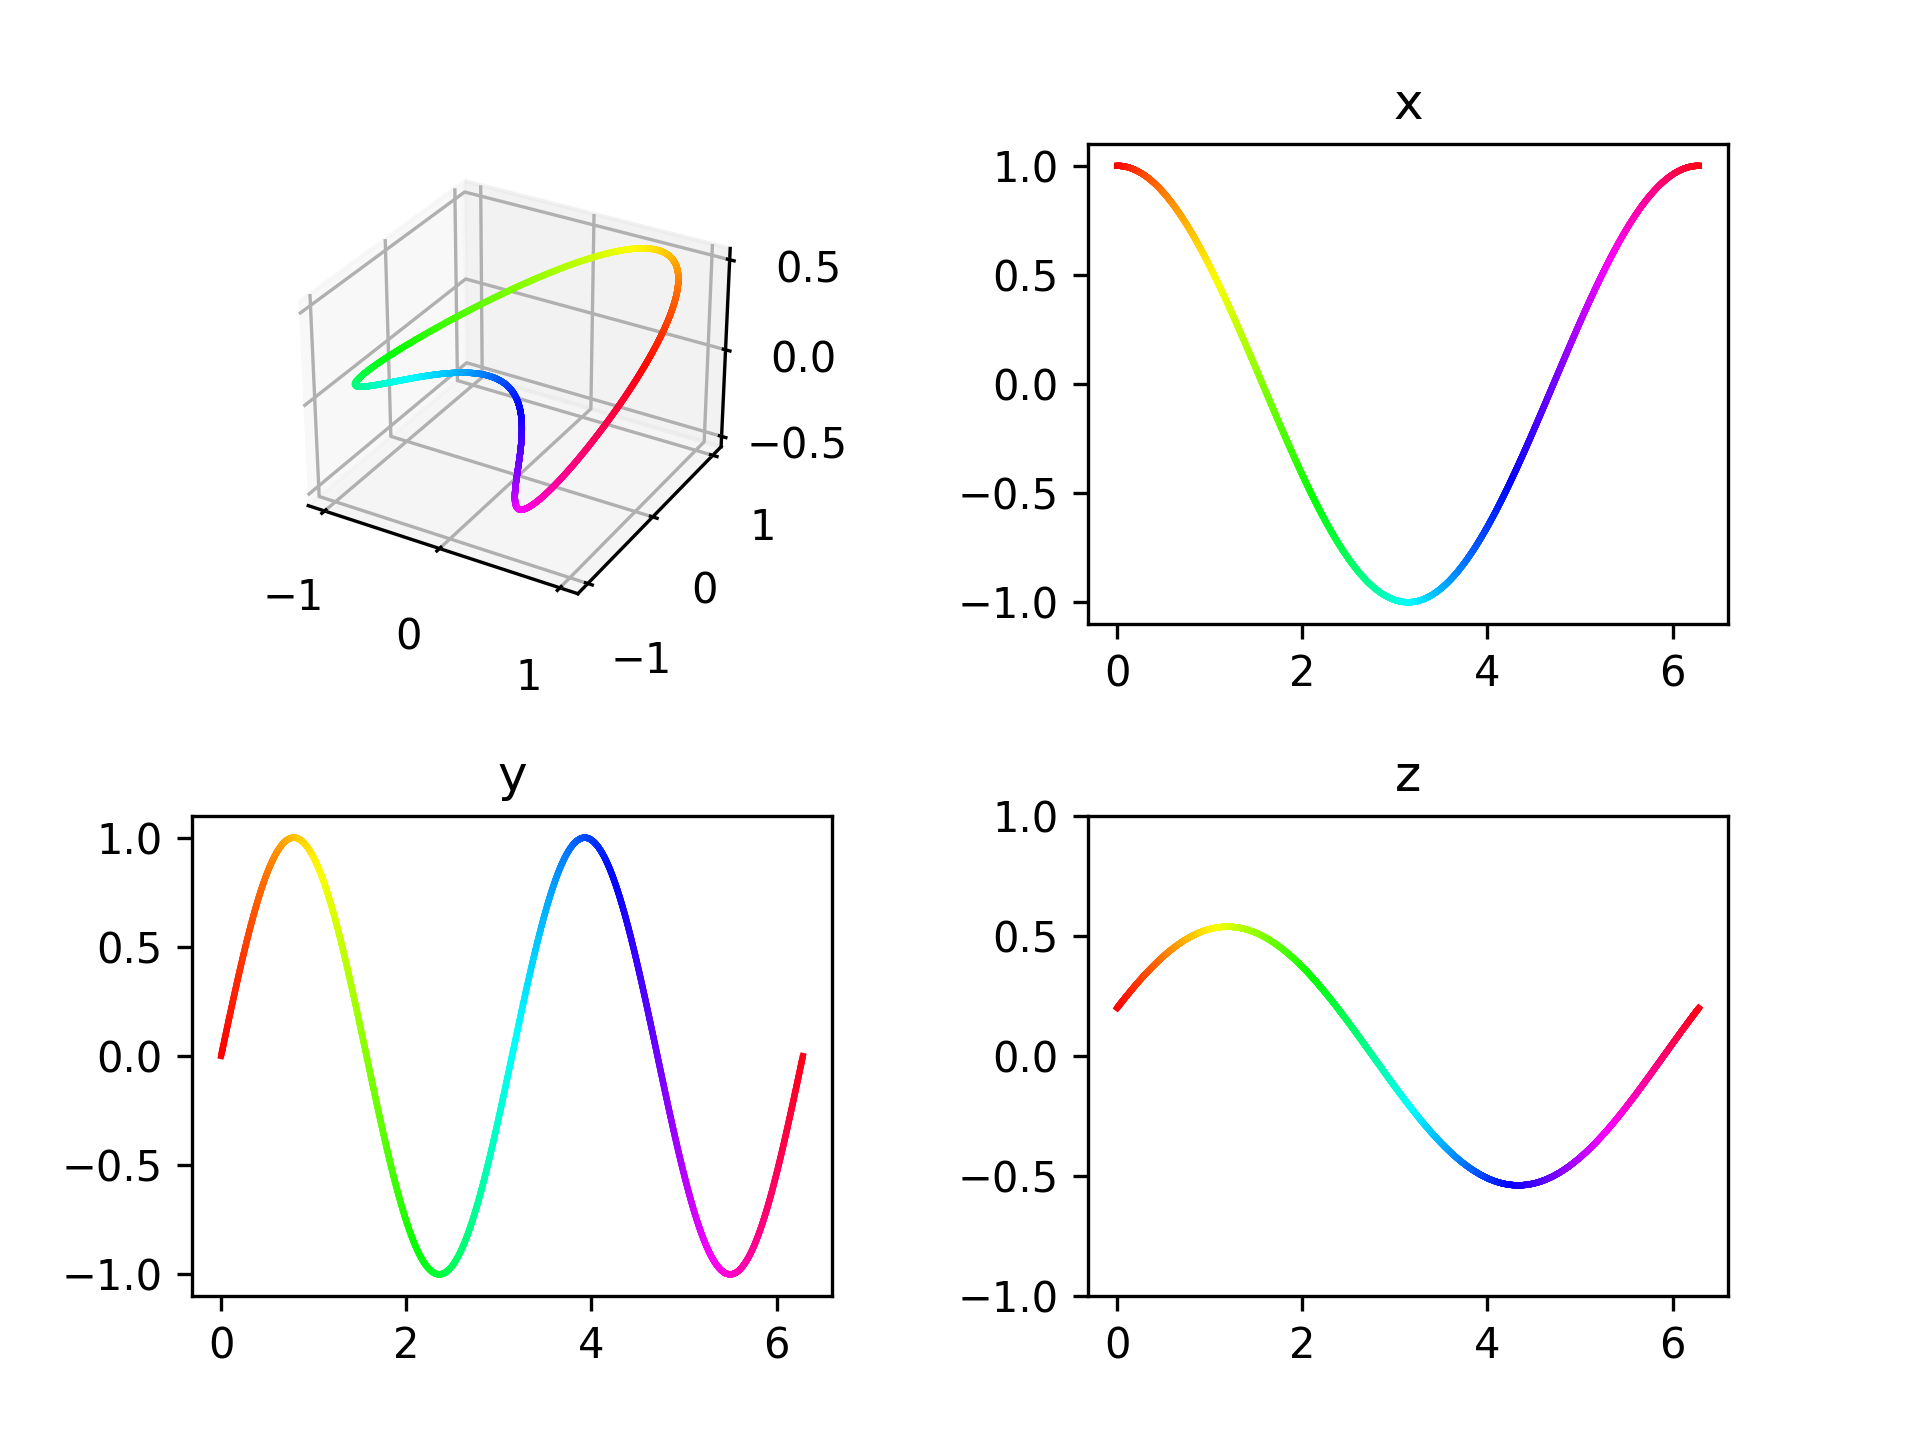
\includegraphics[width=\textwidth]{sections/FourierSeriesImgs/FSProjection}
    \caption{Decomposition of curve $\gammabf\in\mathbb{S}$ into 1D functions in each coordinate.}
    \label{fig: Fourier series decomposition into 1D}
\end{figure}

Now the idea is to truncate the series to order $J > 0$ terms and collect its coefficients,
that is,
\begin{equation*}
    \gammabf(t) \approx \sum_{n=-J}^{J}
    \underbrace{
    \begin{pmatrix}
        c_{1,n} \\
        c_{2,n} \\
        c_{3,n}
    \end{pmatrix}
}_{\cbf_n}
    e^{-int}
\end{equation*}
One may justify the truncation of Fourier series representation by the following remark:
\begin{remark}[Rate of Convergence for Fourier Series\cite{fourierseries}]
    For sufficiently well-behaving $f \in \mathcal{C}^{p-1}$, typically the nonzero coefficients $c_n$ decay as $O\left( \frac{1}{n^{p+1}} \right)$.
    This can be made more rigorous by theorem \ref{thrm: Rate of Convergence of Chebyshev Series},
    and the remark following it.
%\lipsum[1]
\end{remark}
Now, using these coefficients, one could construct the approximate discrete curve $\Gammabf_{N,J}$ of resolution $N \gg J$.
Take the dependent variables for the tangent-point energy to be the coefficients on Fourier series representation:
\begin{equation}
    \mathcal{E}_{\beta}^{\alpha} \left( \gammabf \right)
    \approx
    \mathcal{E}_{\beta}^{\alpha} \left( \gammabf_{J} \right)
    =
    \mathcal{E}_{\beta}^{\alpha} \underbrace{\left( \cbf_{-J}, \cbf_{-J+1}, \cdots, \cbf_{J} \right)}_{3\left( 2J+1 \right) \text{ variables}}
    \approx
    E_{\beta}^{\alpha} \left( \Gammabf_{N,J} \right)
\end{equation}
This time, instead of solving for gradient flow equation,
we use standard methods of minimising a function, such as gradient descent or otherwise \textit{over the $3(2J+1)$ coefficients\footnote{Without loss of generality, one could take $c_{i,0} = 0$ for $i=1,2,3$ as it only determines constant shift of the entire curve, so one actually only needs to consider $6J$ coefficients.}} $\cbf_{-J}, \cbf_{-J+1}, \cdots, \cbf_{J}$.
It is practical to take $N$ to be larger than the resolution for the discrete gradient flow,
as we have will have less variables to minimise over anyways.
The smoothness of the evolving curve follows since it is represented as a finite sum of infinitely smooth function,
so there is no misbehaviour from sharp points as in Figure \ref{fig: L2Derivative}.

\subsubsection{Curves in $\mathbb{L}$}
For $\gammabf$ that is not closed, but rather homeomorphic to a line segment,
it is more natural to use Chebyshev approximation\cite{Trefethen_2020}.
\begin{definition}[Chebyshev Polynomial]
    $n$\textsuperscript{th} Chebyshev polynomial $T_n(x)$ over $\left[ -1,1 \right]$ is defined in the following way:
    \begin{align}
        x &= \frac{1}{2} \left( z+z^{-1} \right) = \cos{\theta} \\
        T_n(x) &= \frac{1}{2}\left( z^n + z^{-n} \right) = \cos{(n\theta)}
    \end{align}
    where $z \in \left\{ z\in\mathbb{C} \middle| |z| = 1 \right\}$.
\end{definition}
For a curve $\gammabf:\left[ -1, 1 \right] \rightarrow \mathbb{R}^3$ such that $\gammabf \in \mathbb{L}$,
there exists a Chebyshev series representation:
\begin{equation}
    \gammabf (t) =
    \underbrace{
    \begin{pmatrix}
        a_{1,0} \\
        a_{2,0} \\
        a_{3,0}
    \end{pmatrix}
}_{\abf_0}
    +
    \sum_{n=1}^{\infty}
    \underbrace{
    \begin{pmatrix}
        a_{1,n} \\
        a_{2,n} \\
        a_{3,n}
    \end{pmatrix}
}_{\abf_n}
    T_n (t)
\end{equation}
where $T_n (t)$ is the $n$\textsuperscript{th} Chebyshev polynomial.
The coefficients $\left\{ a_{i,n} \right\}$ are given by:
\begin{equation}
    a_{i,n} = \frac{2}{\pi} \int_{-1}^{1} \frac{\gamma_i(t) T_n(t)}{\sqrt{1-t^2}} \intd t
\end{equation}
for $i = 1, 2, 3$.

We again approximate $\gammabf$ by truncating the Chebyshev series up to order $J$ term,
which we justify by the following theorem for Chebyshev series:
\begin{theorem}[Rate of Convergence for Chebyshev Series\cite{Trefethen_2020}]
    \label{thrm: Rate of Convergence of Chebyshev Series}
    For $f:\left[ -1,1 \right]\rightarrow \mathbb{R}$ such that its derivatives through $f^{(p-1)}$ are absolutely continuous, and $f^{(p)}$ is of bounded variation, then the nonzero coefficients decay as $O\left( \frac{1}{n^{p+1}} \right)$ and the 2-norm error of interpolants and truncations decay as $O\left( \frac{1}{n^p} \right)$.
\end{theorem}
\begin{remark}
    There is actually a way in a sense that Chebyshev series and Fourier series are equivalent, which is outlined in \cite{Trefethen_2020}.
    The remark of rate of convergence of Fourier series can be posed, hence, equivalently to this theorem.
\end{remark}

Then, interpret the tangent-point energy to dependent on its coefficients.
\begin{equation}
    \mathcal{E}_{\beta}^{\alpha} \left( \gammabf \right)
    \approx
    \mathcal{E}_{\beta}^{\alpha} \left( \gammabf_{J} \right)
    =
    \mathcal{E}_{\beta}^{\alpha} \underbrace{\left( \abf_{0}, \abf_{1}, \cdots, \abf_{J} \right)}_{3\left( J+1 \right) \text{ variables}}
    \approx
    E_{\beta}^{\alpha} \left( \Gammabf_{N,J} \right)
\end{equation}
This time, the tangent-point quadrature is taken as the one in Appendix \ref{sct: Curves in L}.

\subsubsection{Sample Points and Time Complexity}
While approximation via series reduces the number of dimensions to reduce the tangent-point energy over,
in order to compute the derivative (against coefficients),
one still needs to use quadrature, meaning, one needs to take $N$ sample points.

Because we have captured the function that describes the curve rather than points,
there is more flexibility to either sample/resample points as needed,
simply by varying the parameter for the sample points.

There are natural choice of sample points for curves in $\mathbb{S}$ and $\mathbb{L}$.
\begin{itemize}
    \item For a curve $\gammabf \in \mathbb{S}$, the natural choice of sample points are points of which the parameter values are equispaced on the interval $\left[ 0,2\pi \right)$.
        \begin{equation}
\left\{ \gammabf(t) \middle| t = \frac{2\pi}{N}j, j \in \left\{ 0, 1, \cdots, N-1 \right\} \right\}
        \end{equation}
    \item For a curve $\gammabf \in \mathbb{L}$, the natural choice of sample points are Chebyshev points on the interval. (Figure \ref{fig: Chebyshev Points})
        \begin{equation}
            \left\{ \gammabf(t) \middle| t = \cos \left( \frac{j \pi}{N} \right), j \in \left\{ 0, 1, \cdots, N \right\} \right\}
        \end{equation}
Use of Chebyshev points may aid in avoiding Runge phenomenon\cite{Trefethen_2020}.
\end{itemize}
\begin{figure}[tbp]
    \centering
    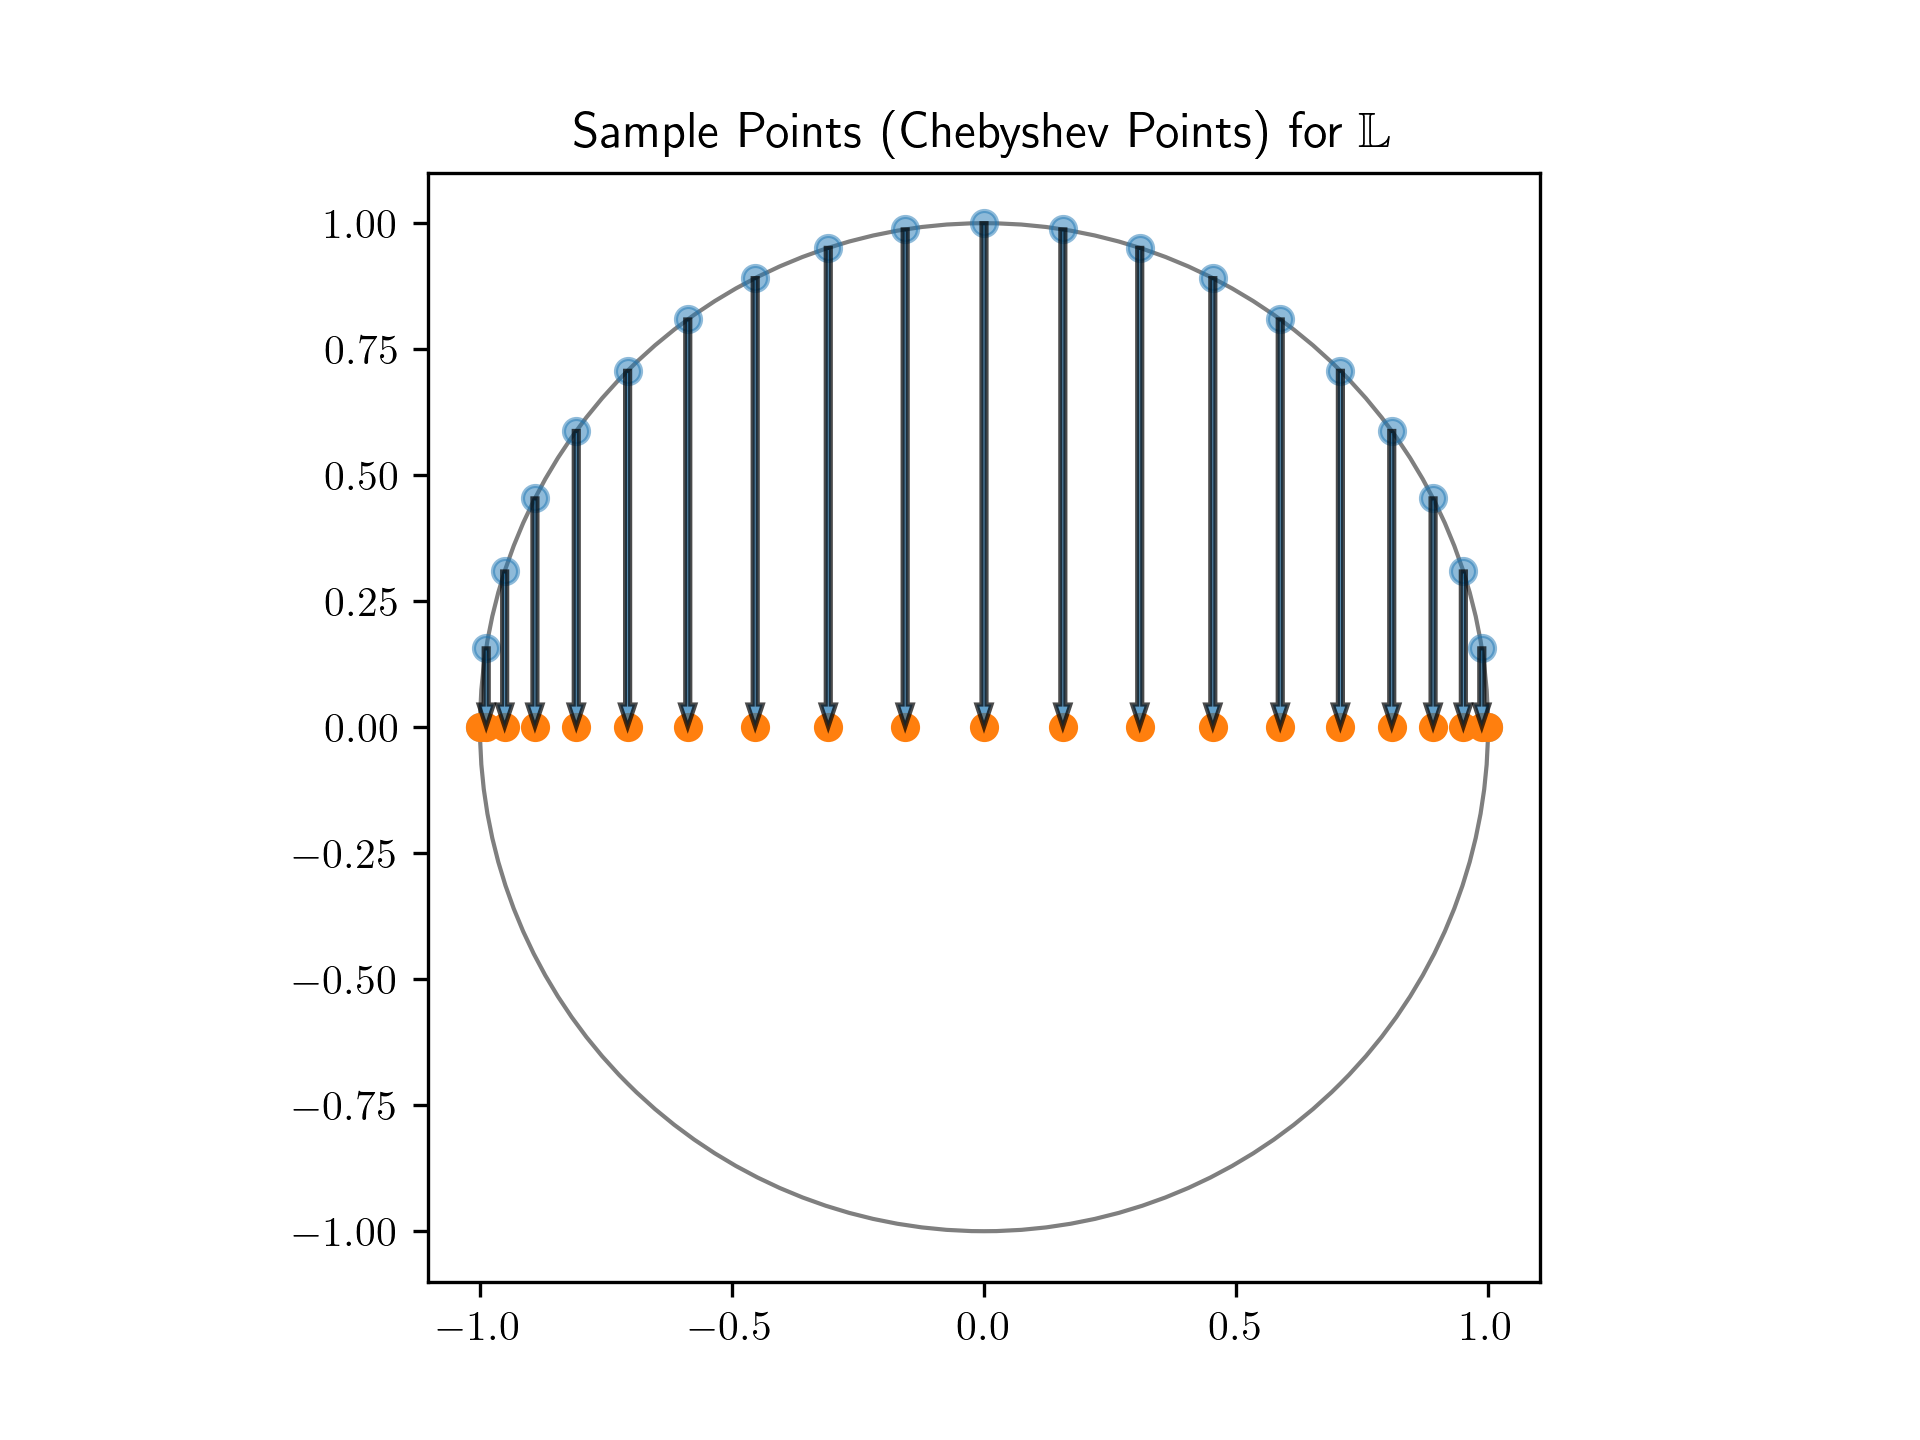
\includegraphics[width=\textwidth]{sections/FourierSeriesImgs/ChebyshevPoints}
    \caption{Chebyshev points are acquired from projecting equally spaced points on a unit circle to the $x$-axis.
    Note that the ``density'' of points is the highest at the ends.}
    \label{fig: Chebyshev Points}
\end{figure}
\begin{figure}[tbp]
    \centering
    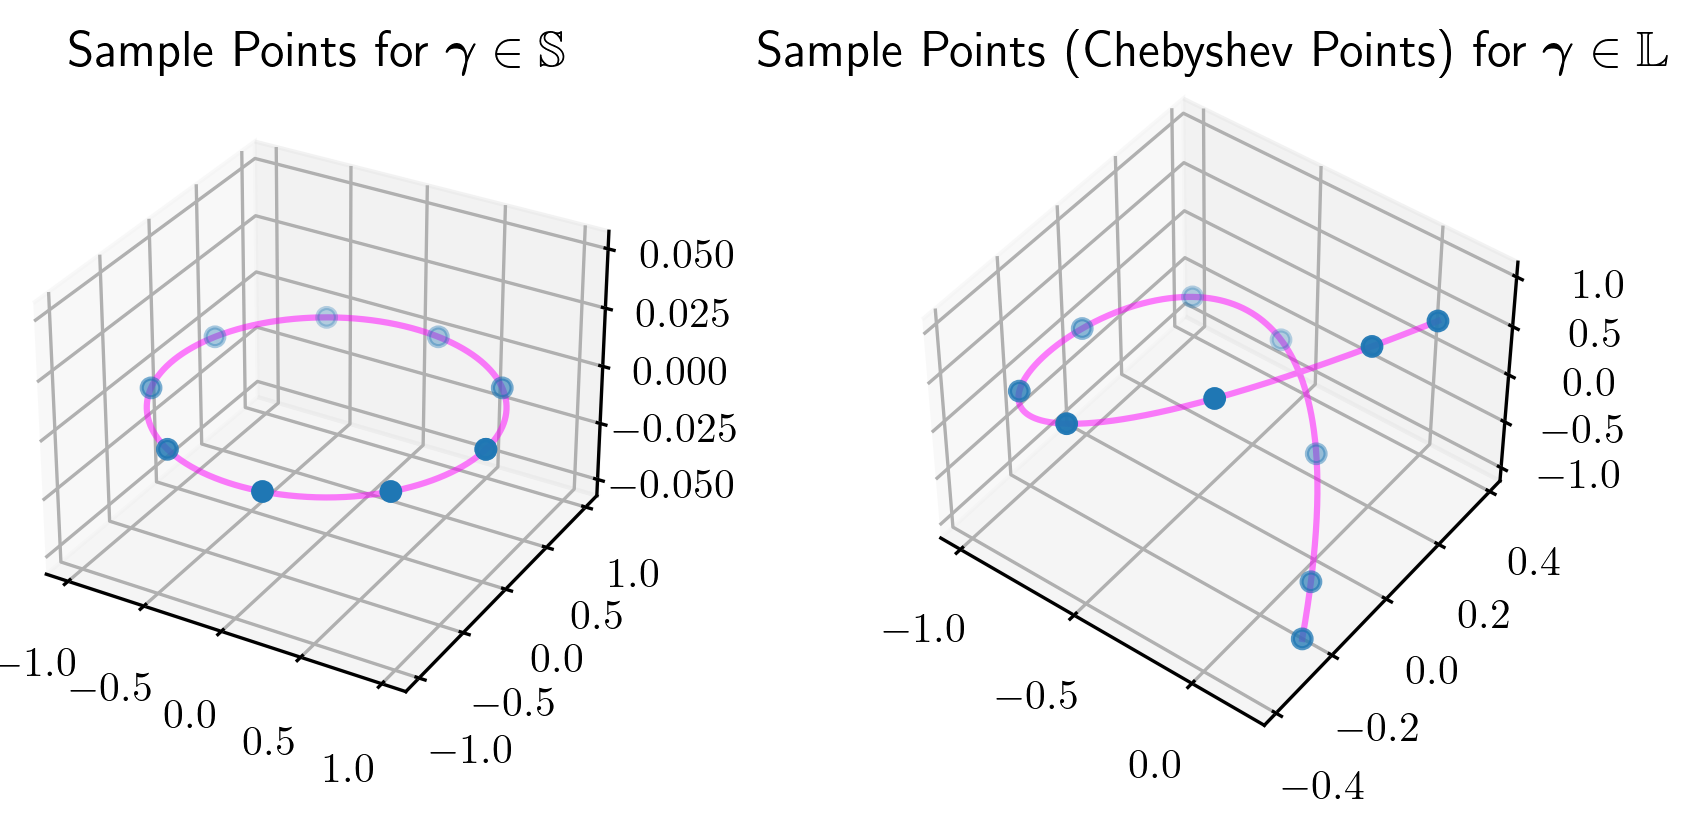
\includegraphics[width=\textwidth]{sections/FourierSeriesImgs/SamplePointsOnCurves}
    \caption{Natural sample points on $\gammabf \in \mathbb{S}$ and $\gammabf \in \mathbb{L}$}
\end{figure}

Note that keeping $N$ constant during evolution allows one to optimise the generation/computation of sample points.
For example, for $\gammabf \in \mathbb{S}$, the points on the discretised curve $\Gammabf_{N,J}^k$:
\begin{align}
    \Gammabf_{N,J}^k [j] &= \xbf_{j}^{k} = \sum_{n=-J}^{J} \cbf_{n} e^{i \frac{2\pi}{N}n j} & j=0,1,\cdots,N-1
    \label{equ: DFT}
\end{align}
By using modified FFT\cite{5213896}, one could reduce the cost from $O\left( NJ \right)$ to $O \left( J \log N \right)$.
Also, because the tangent-point energy of the truncated curve $\mathcal{E}_{\beta}^{\alpha} \left( \gammabf_{J} \right)$ involves integral which the integration variable is independent from the coefficients $\cbf_n$,
one could, in theory, directly compute derivative by differentiating under the integral sign (which turns out to be a messy computation, but possible),
or one could use central difference scheme to approximate it;
because one only needs to compute $3J$ derivatives\footnote{Order $0$ terms do not contribute as tangent-point energy is shift-invariant, hence derivative with respect to those coefficients are identically zero.}
instead of $3N \gg 3J$ derivatives, this can be a practical approach.
With latter approach to compute derivative, this would result in $O\left( J^3 + J \log N \right)$ operations per time step.
Because $J$ does not need to be large at all\footnote{Instead of storing a unit circle with, say $N = 90$ points, one technically only needs $J=1$ to do the same.},
and in fact, assuming that the higher order coefficients decay fast enough,
one could ``deflate'' the problem by truncating the series further later,
the ``practical cost'' (assuming $J$ is of constant order) can be expressed as $O\left( \log N \right)$ with this approach.

Similar analysis can be done with curves in $\mathbb{L}$ as the evaluation of Chebyshev series can also be improved using FFT\cite{Trefethen_2020}.


\begin{figure}[tbp]
    \centering
    \begin{subfigure}[b]{0.5\textwidth}
        \centering
        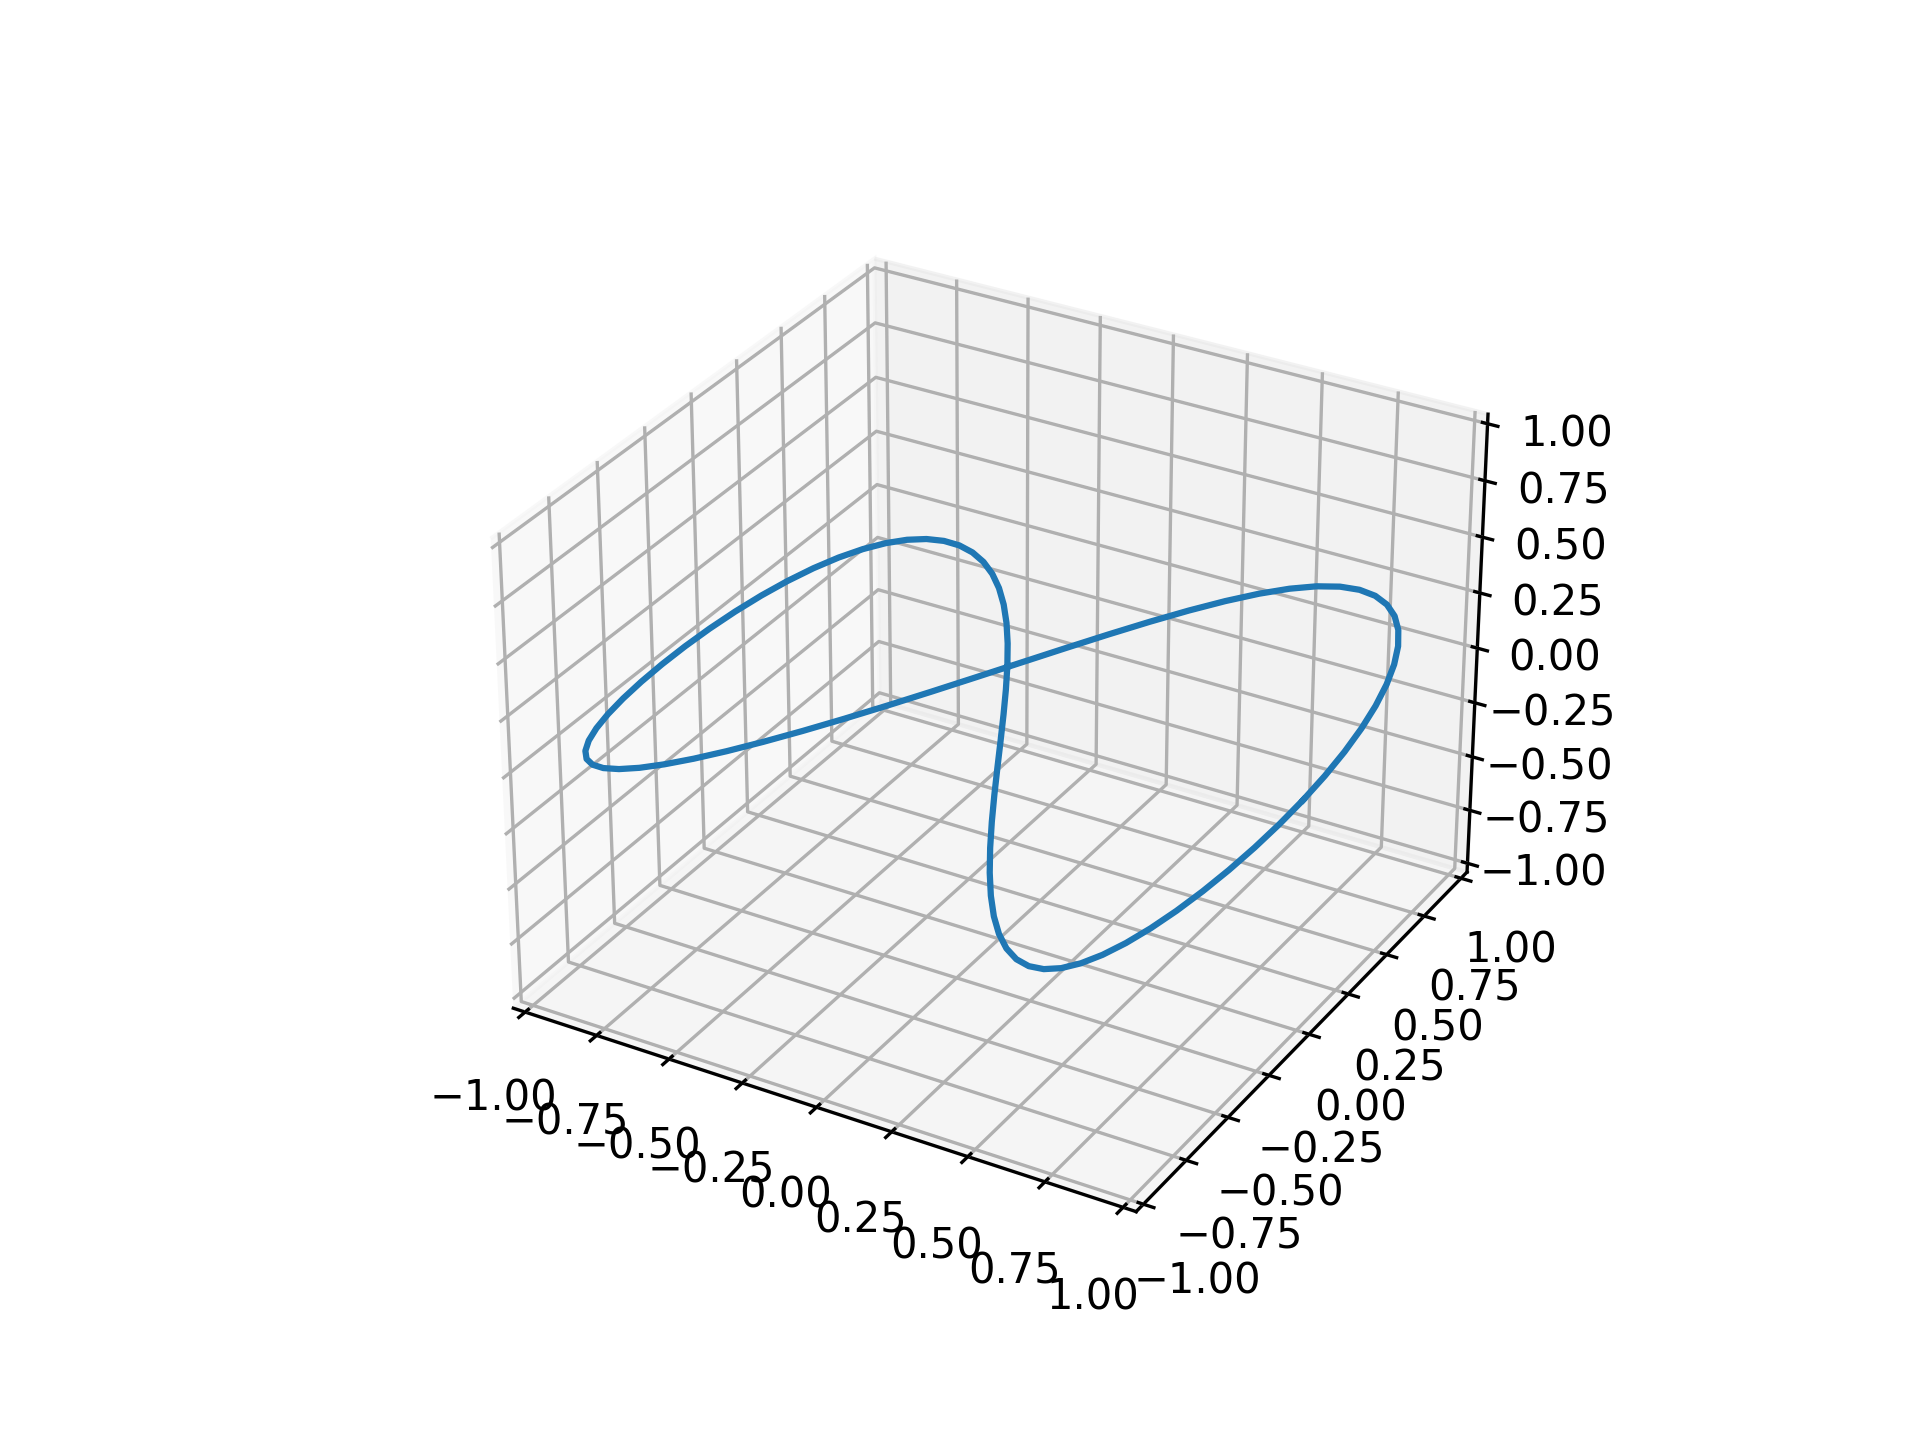
\includegraphics[width=\textwidth]{sections/FourierSeriesImgs/Fourier0}
    \end{subfigure}
    \begin{subfigure}[b]{0.45\textwidth}
        \centering
        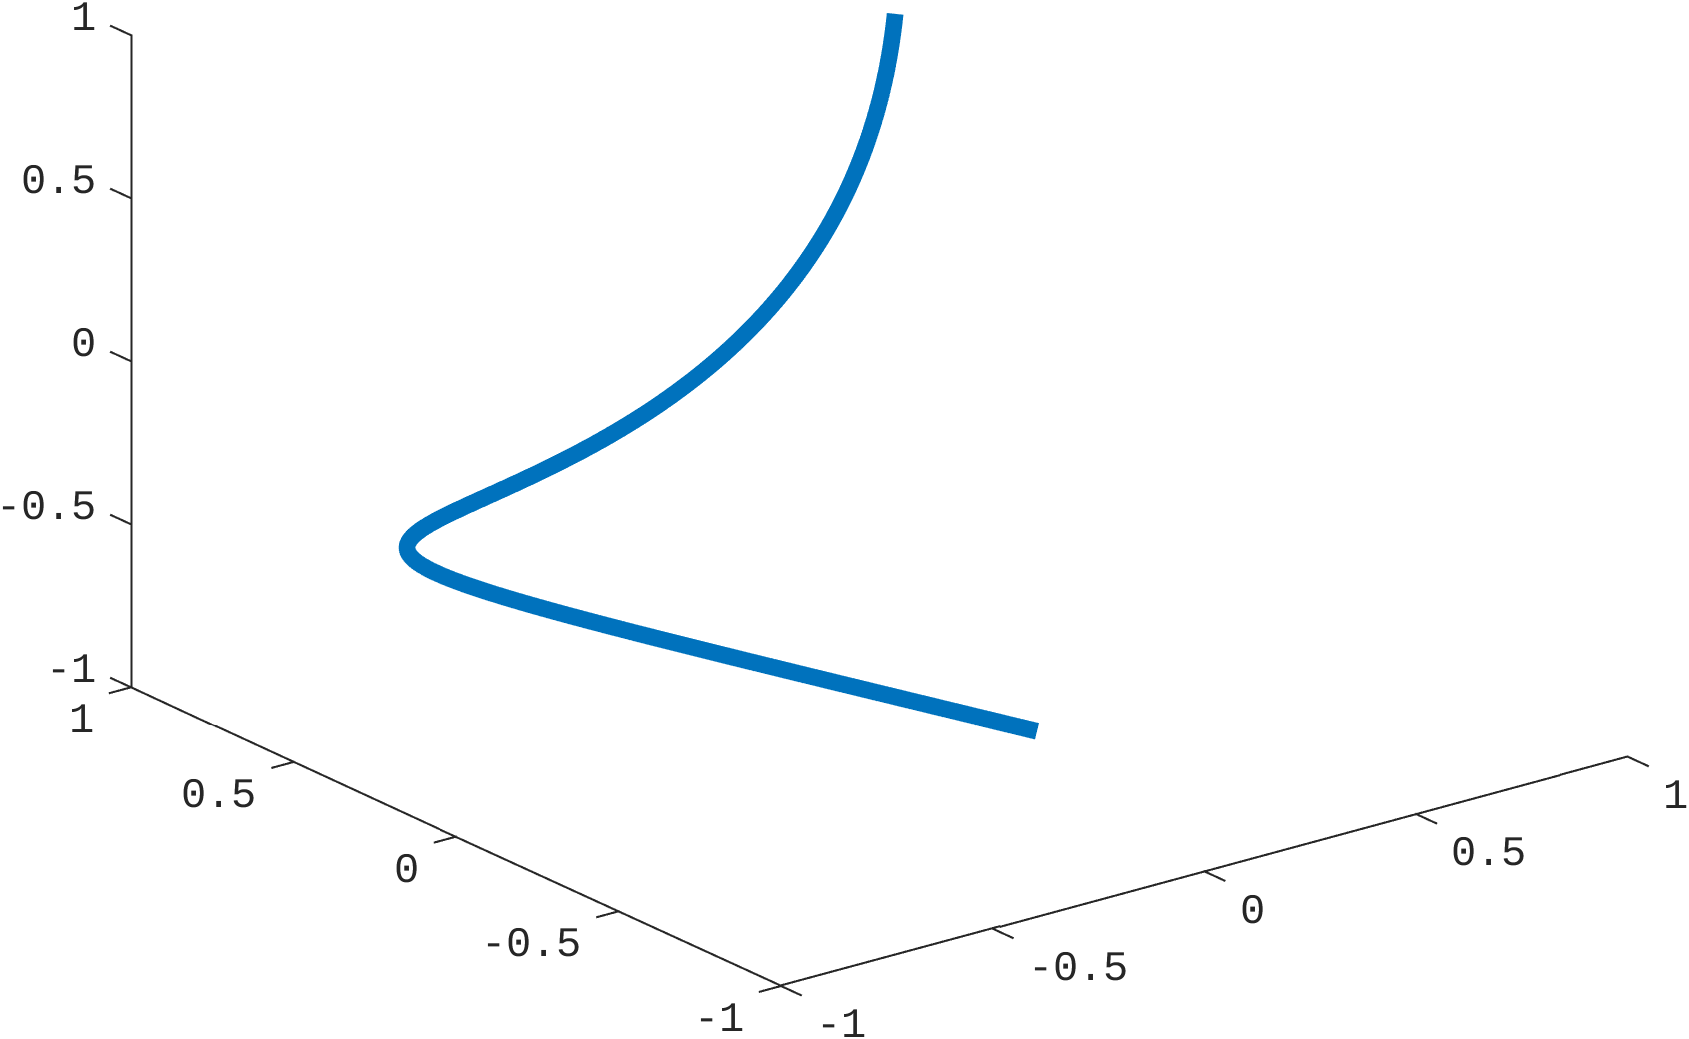
\includegraphics[width=\textwidth]{sections/FourierSeriesImgs/Chebyshev0}
    \end{subfigure}
    \begin{subfigure}[b]{0.5\textwidth}
        \centering
        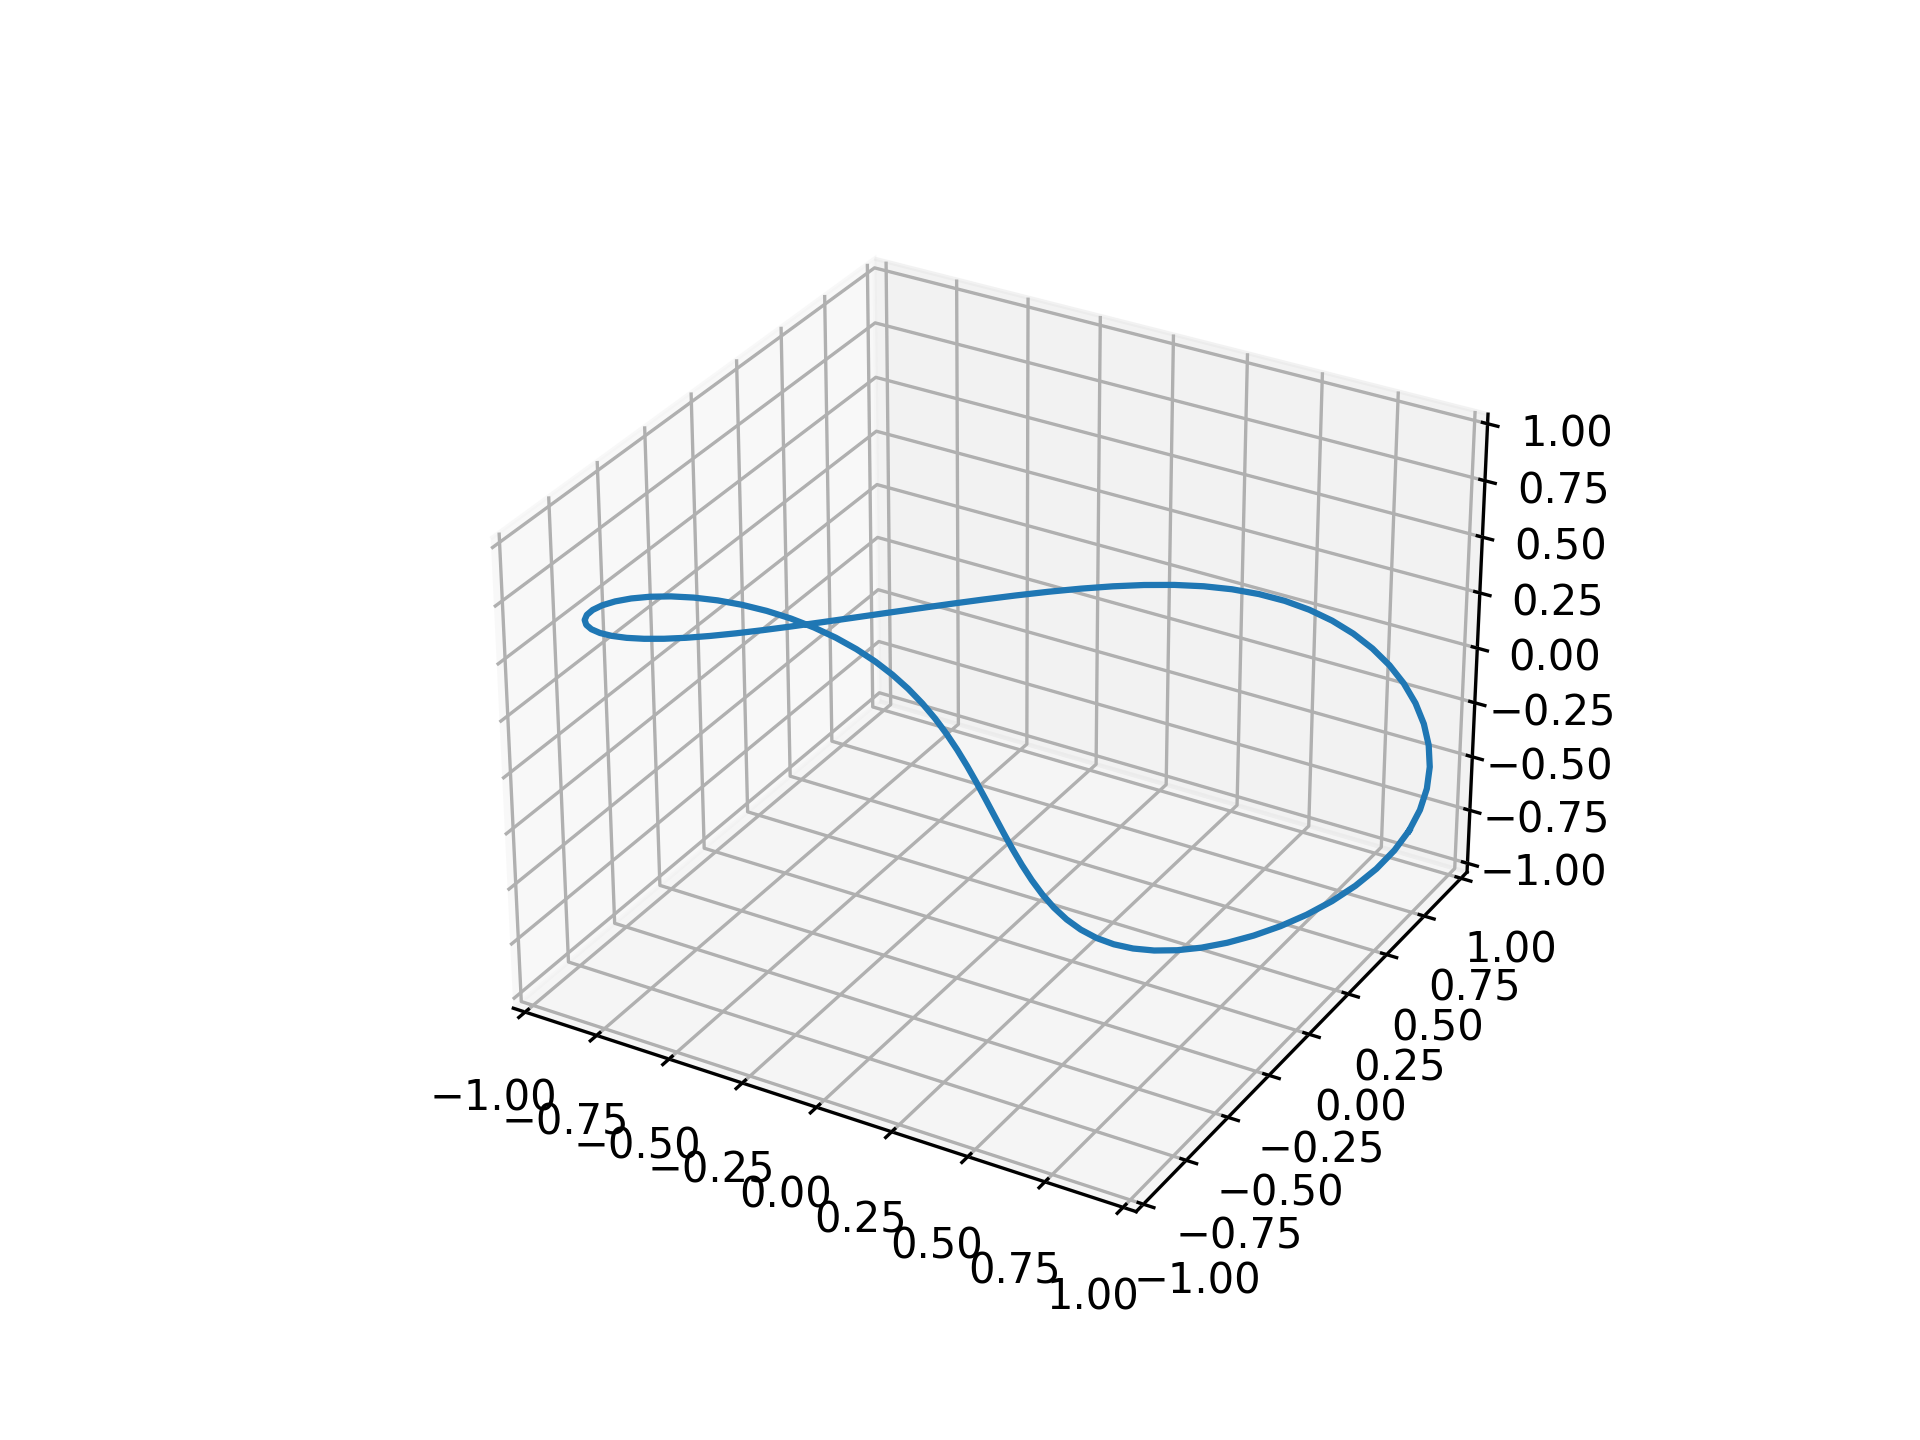
\includegraphics[width=\textwidth]{sections/FourierSeriesImgs/Fourier1}
    \end{subfigure}
    \begin{subfigure}[b]{0.45\textwidth}
        \centering
        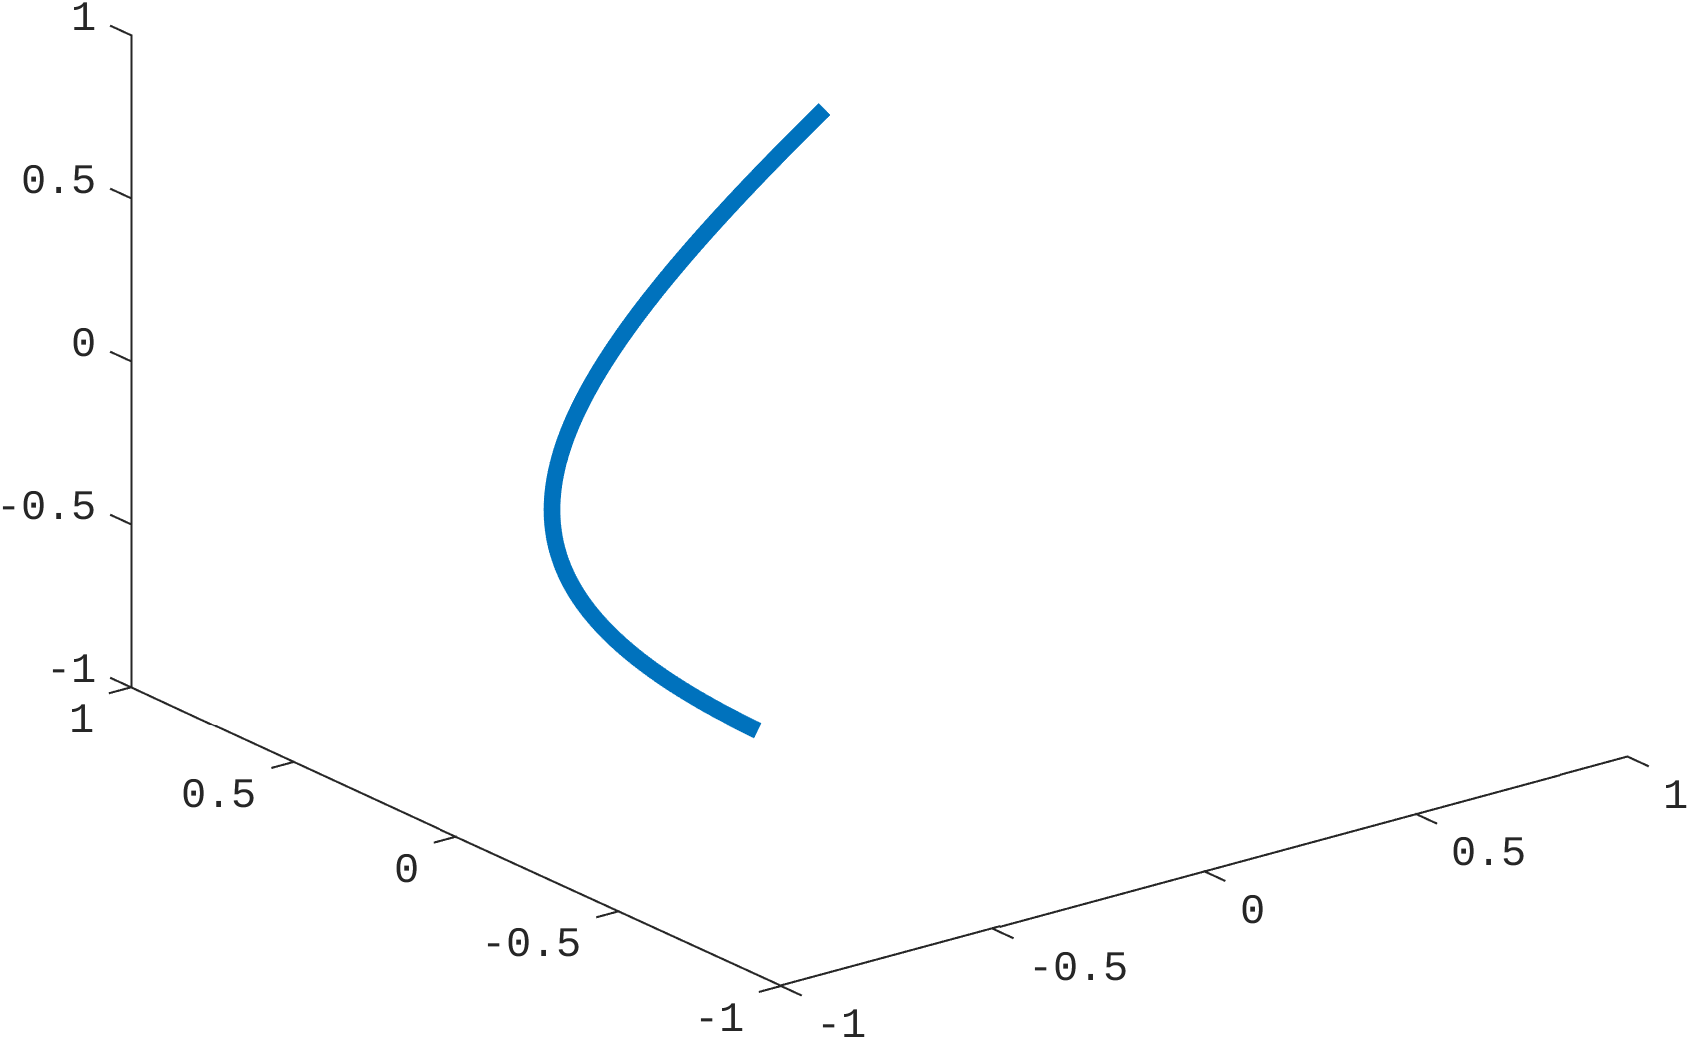
\includegraphics[width=\textwidth]{sections/FourierSeriesImgs/Chebyshev1}
    \end{subfigure}
    \begin{subfigure}[b]{0.5\textwidth}
        \centering
        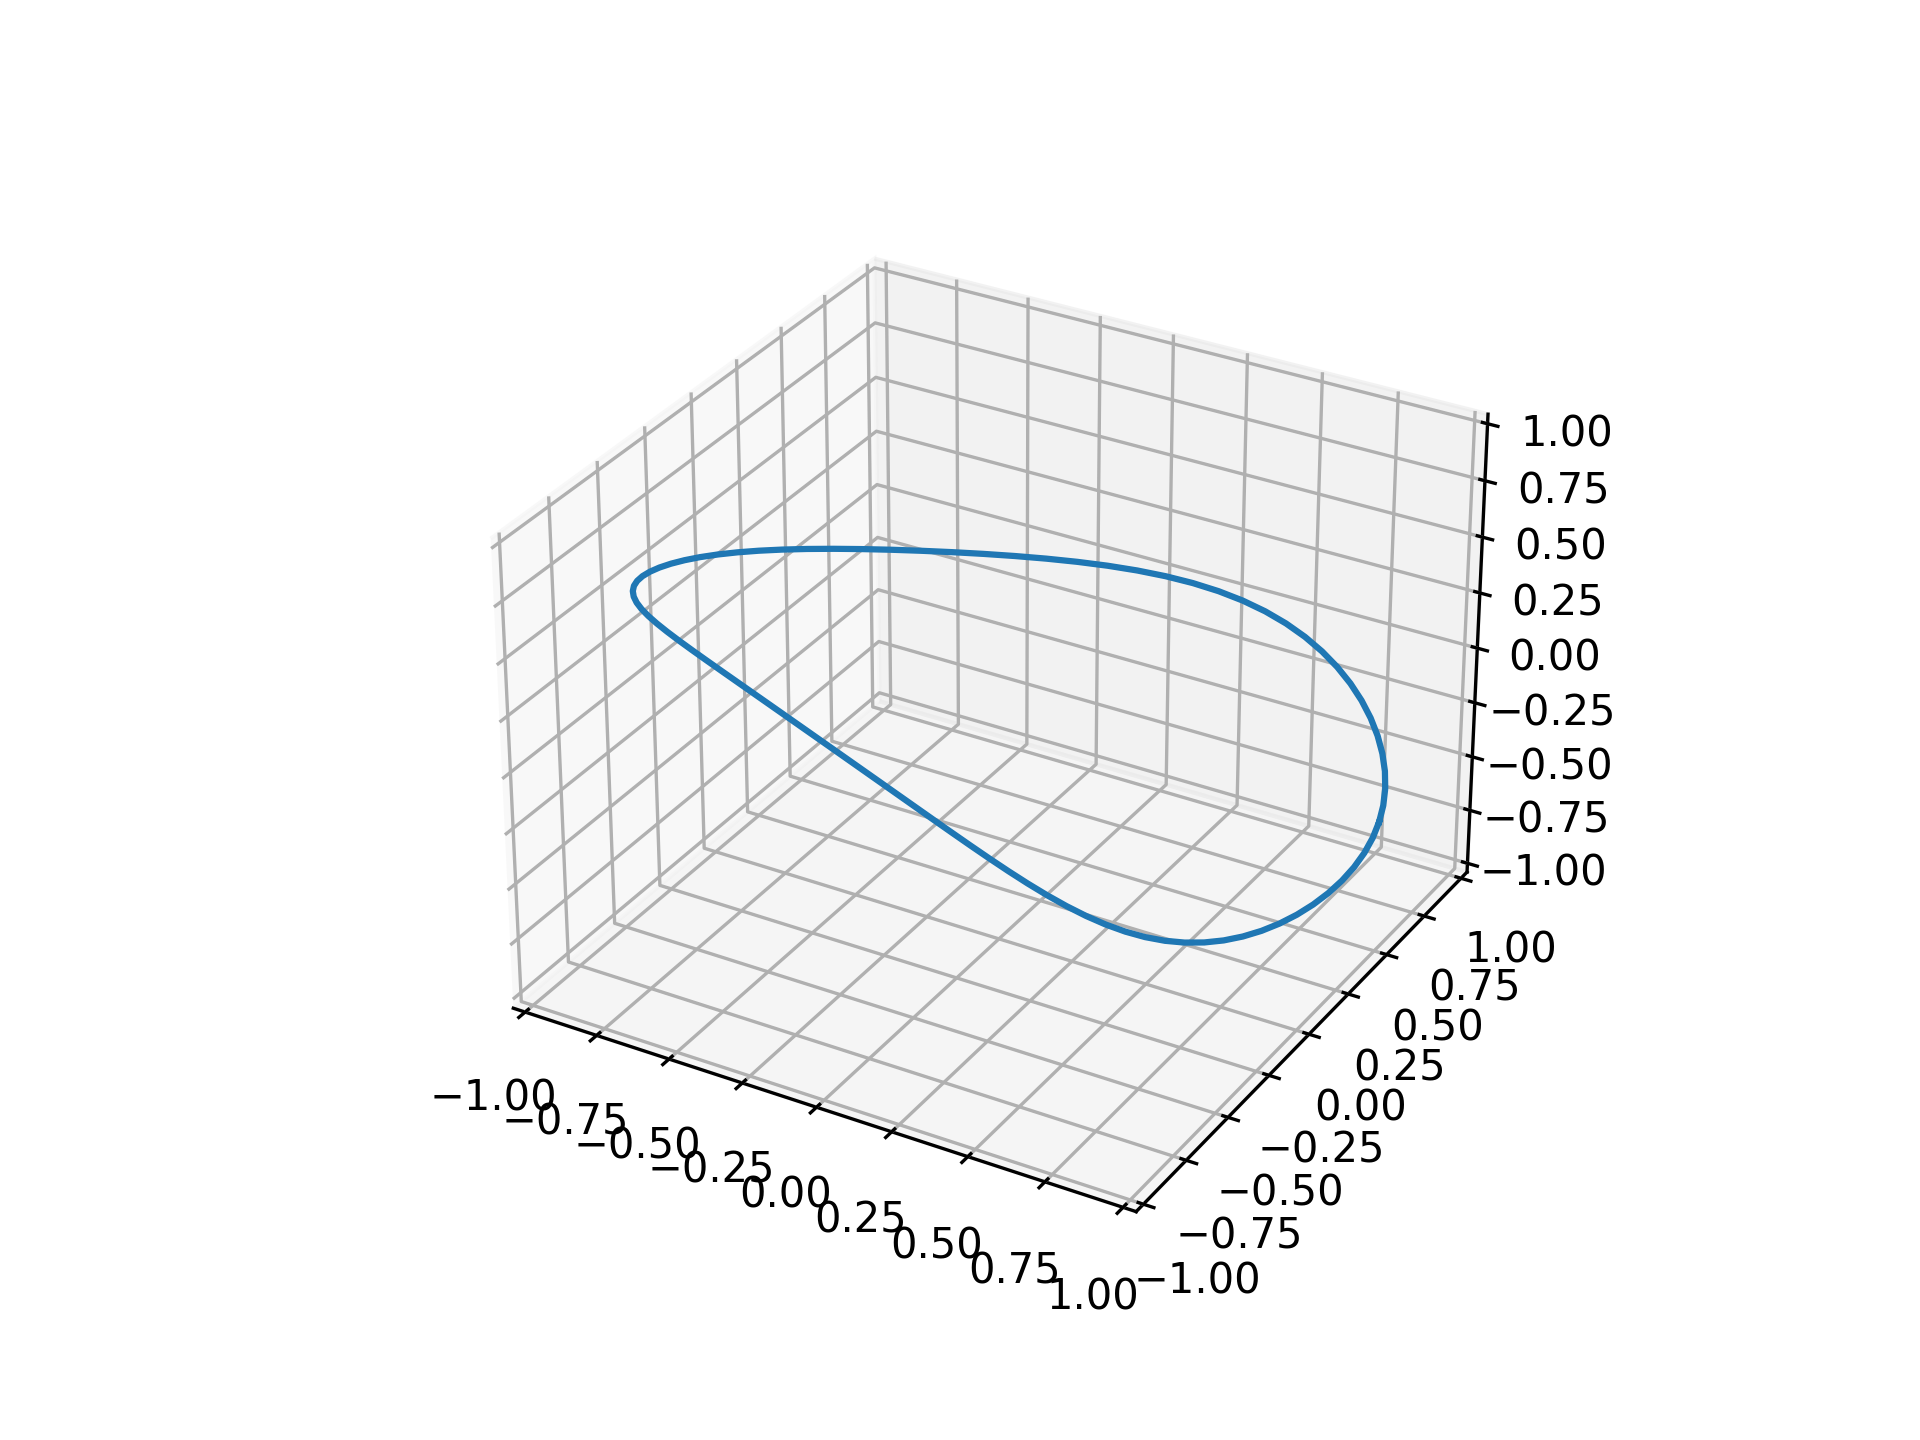
\includegraphics[width=\textwidth]{sections/FourierSeriesImgs/Fourier2}
    \end{subfigure}
    \begin{subfigure}[b]{0.45\textwidth}
        \centering
        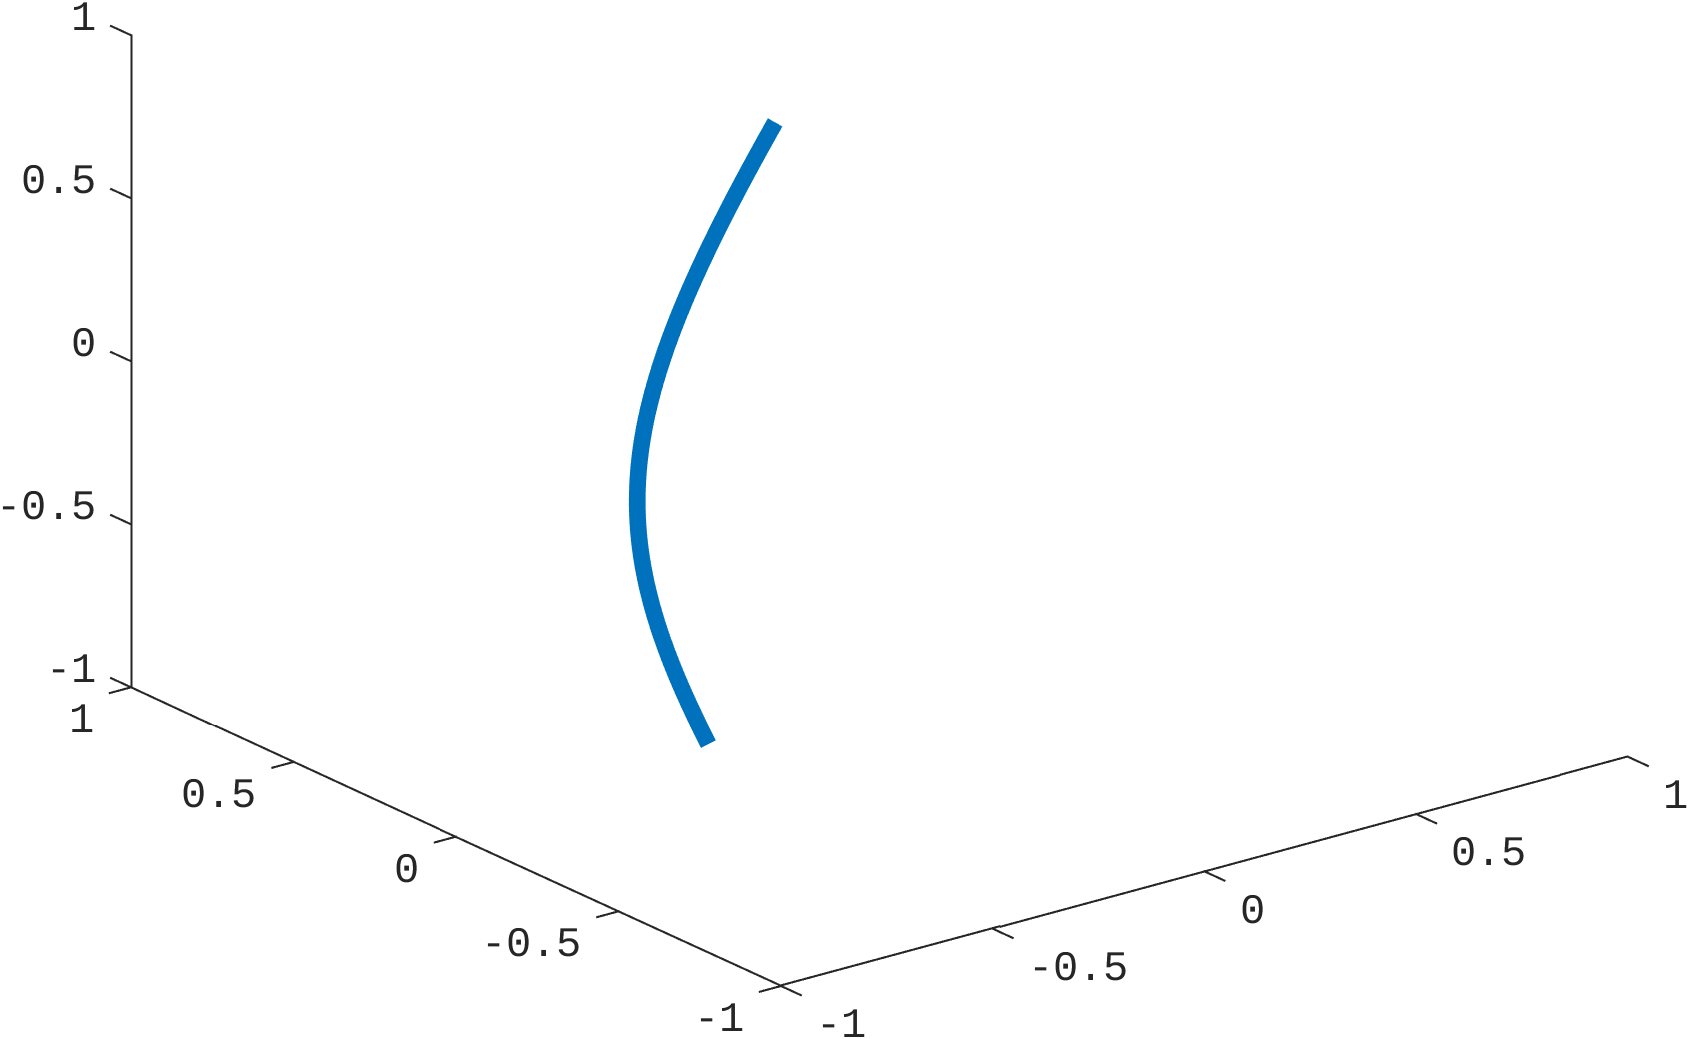
\includegraphics[width=\textwidth]{sections/FourierSeriesImgs/Chebyshev2}
    \end{subfigure}
    \caption{Evolution of $\gammabf \in \mathbb{S}$ and $\gammabf \in \mathbb{L}$.}
\end{figure}
The full algorithm with deflation is outlined in Algorithm \ref{alg: Energy Reduction via Approximation Theory with Deflation}.
As demonstrated in Figure \ref{fig: UnknottingEnergiesProgress},
this method can indeed be practical.

\begin{algorithm}[tbp]
    \caption{Fixed Step-size Energy Reduction via Approximation Theory with Deflation}
    \label{alg: Energy Reduction via Approximation Theory with Deflation}
    \begin{algorithmic}
        \State Choose $J$. (Depends on the complexity of the initial curve.)
        \State Let $k=0$.
        \State Choose $M > 0$, the number of time steps.
        \State Choose $N > J$, the resolution of the curve to generate.
        \State Choose $0 < \epsilon \ll 1$, the tolerance for deflation.
        \State Choose $0 < \Delta T \ll 1$, the fixed step size.
        %\Comment{One could easily conceive an algorithm which the time step changes.}

        \State Given initial curve $\gammabf$ or initial set of sample points $\Gammabf$, find a series approximation up to order $J$.
        \While{$k < M$}
        \State Compute sample points $\Gammabf_{N,J}^k$ as in (\ref{equ: DFT}) via FFT.
        \State Compute $\nabla_{\cbf} E_{\beta}^{\alpha} \left( \Gammabf_{N,J}^k \right)$ exactly or approximately, where the $\nabla_{\cbf}$ is gradient operator over all the coefficients of the series.
        \Comment{$\cbf$ is the array of coefficients.}
        \State Evolve a time step by $\cbf \leftarrow \cbf - \Delta T \nabla_{\cbf} E_{\beta}^{\alpha} \left( \Gammabf_{N,J}^k \right)$.
        \If{$\exists j \suchthat \forall i \geq j$, the modulus of the order $i$ coefficient is less than $\epsilon$}
        \State Truncate the series to order $j-i$ term.
        \State $J \leftarrow j-i$.
        \Comment{Deflation: reduced $J$, so expect a speedup in computation.}
        \EndIf
        \State $k \leftarrow k+1$
        \EndWhile
    \end{algorithmic}
\end{algorithm}

\begin{figure}[tbp]
    \centering
    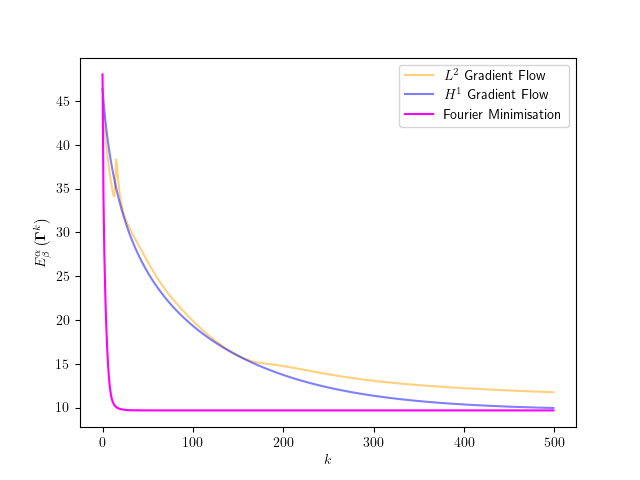
\includegraphics{sections/conclusionImgs/UnknottingEnergiesProgress}
    \caption{The method of minimising function can be much faster than using the gradient flow.}
    \label{fig: UnknottingEnergiesProgress}
\end{figure}

\end{document}
